%%%%%%%%%%%%%%%%%%%%%%%%%%%%%%%%%%%%%%%%%%%%%%%%%%%%%%%%%%%%%%%%%%%%%%
%
% Institut für Rechnergestuetzte Automation
% Forschungsgruppe Industrial Software
% Arbeitsgruppe ESSE
% http://security.inso.tuwien.ac.at/
% lva.security@inso.tuwien.ac.at
%
% Version 2012-10-17
% 
%%%%%%%%%%%%%%%%%%%%%%%%%%%%%%%%%%%%%%%%%%%%%%%%%%%%%%%%%%%%%%%%%%%%%%

\documentclass[12pt,a4paper,titlepage,oneside]{scrartcl}
\usepackage{esseProtocol}

%%%%%%%%%%%%%%%%%%%%%%%%%%%%%%%%%%%%%%%%%%%%%%%%%%%%%%%%%%%%%%%%%%%%%%
%
% FOR STUDENTS
%
%%%%%%%%%%%%%%%%%%%%%%%%%%%%%%%%%%%%%%%%%%%%%%%%%%%%%%%%%%%%%%%%%%%%%%

% Group number or "0" for Lab0
\newcommand{\gruppe}{5}
% Date
\newcommand{\datum}{05.06.2013}
% valid values: "Lab0", "Lab1" (be sure to use Uppercase for first character)
\newcommand{\lab}{Lab1}

% name of course, for example: "IT Security in Large IT Infrastructures", "Security for Systems Engineering", "Introduction to Security"
\newcommand{\lvaname}{IT Security in Large IT Infrastructures}
% number of course, for example: "183.633", "183.637", "183.594"
\newcommand{\lvanr}{183.633}
% year and term, for example: "SS 2012", "WS 2012", "SS 2013", etc.
\newcommand{\semester}{SS 2013}

% Student data in Lab0 or 1. student of group in Lab1
\newcommand{\studentAName}{Michael Heil}
\renewcommand{\studentAMatrnr}{0826358}
\newcommand{\studentAEmail}{e0826358@student.tuwien.ac.at}

% 2. student of group in Lab1, for Lab0 or if your group has less students, remove this 3 lines
\newcommand{\studentBName}{Lukas Puschmann}
\renewcommand{\studentBMatrnr}{0825354}
\newcommand{\studentBEmail}{e0825354@student.tuwien.ac.at}

% 3. student of group in Lab1, for Lab0 or if your group has less students, remove this 3 lines
\newcommand{\studentCName}{Dominik Amon}
\renewcommand{\studentCMatrnr}{1228536}
\newcommand{\studentCEmail}{e1228536@student.tuwien.ac.at}


%%%%%%%%%%%%%%%%%%%%%%%%%%%%%%%%%%%%%%%%%%%%%%%%%%%%%%%%%%%%%%%%%%%%%%
%
% DO NOT CHANGE THE FOLLOWING PART
%
%%%%%%%%%%%%%%%%%%%%%%%%%%%%%%%%%%%%%%%%%%%%%%%%%%%%%%%%%%%%%%%%%%%%%%

\newcommand{\dokumenttyp}{Report \lab}

\begin{document}

\maketitle
\setcounter{section}{0}
\setcounter{tocdepth}{2}
\tableofcontents

%%%%%%%%%%%%%%%%%%%%%%%%%%%%%%%%%%%%%%%%%%%%%%%%%%%%%%%%%%%%%%%%%%%%%%
%
% CONTENT OF DOCUMENT STARTS HERE
%
%%%%%%%%%%%%%%%%%%%%%%%%%%%%%%%%%%%%%%%%%%%%%%%%%%%%%%%%%%%%%%%%%%%%%%

\section{Safety Objectives}
Security is the core requirement to this software system. In this chapter we will list and explain the safety objectives of the system as a whole as well as their individual implications to the separate components.

\subsection{Authorization}
Despite the fact that authorization represents the basic functionality of this system, only passing successful authorization attempts is an important goal of our system, it is also an important non-functional issue concerning the communication of the different components themselves. Consequently, all components, especially those outside of our immediate control, but also those within system boundaries are subjects to strict authorization.

A strategy to achieve this goal is to follow the \emph{complete mediation} design principle, which states that every request needs to be verified separately, instead of keeping a cached authorization result. This technique requires more performance but is a must in secure environments.

\subsection{Authenticity}
Similar to \emph{authorization}, authenticity is important for intra- and inter-communication of all components. To ensure authenticity, the \emph{complete mediation} principle provides support for a comprehensive certificate-based authentication system. The used certificates are managed and replaced in regular intervals.

The most vulnerable spots of the system are the external interfaces of the \emph{Authorization and Object Management}. An intruder could gain information about access rights (confidentiality) or change data (integrity). Therefore, it is important to impose a strict authentication and authorization policy.

Functional authentication will be realized using an RFID-chip (similar to the electronic passport). Each employee or user, who wishes to gain access to the system, has to carry one. In normal authentication situations, the person who wants to authorize at the system has to put the chip onto or in front of a reader device and additionally provide a password in order to make the tag communicate with the station. To prevent exploitation of stolen chips, passwords for chips should be changed at least once a year. The holder of the chip is notified about that requirement  on the terminals in time. He/she exchanges the password on his/her own special chip management station. During the process of a password change the certificate is renewed as well. If a chip is stolen or lost there will be a possibility to cancel a chip and make it unusable for further authentications (similar to credit cards).

For critically secured objects an additional iris-scan will be conducted. The scanned data will then be compared to the data stored in the database. The exact procedure will be described in detail in following chapters. Depending on the requirements of the client, the entry of a zone can be protected by a double door system only one person can pass each time.

In general, no component in the system must ever trust any component from beyond the border. The threat of the possibility that components could have been replaced or reconfigured in malicious ways is constantly present.

\subsection{Integrity}
Data integrity is guaranteed at some level by the rigid authentication and authorization mechanisms present within and around the system. Naturally, this goal plays an important role wherever data is stored (which is the \emph{Auditing} and \emph{Authorization and Object Management} component in this system). Checksums will provide means for detecting illegitimate changes to the data. When the authorization storage is kept redundantly, changes to single instances can easily be detected  (see later chapters) .

The most important security measure against alteration of data is the implementation of encryption protocols for all communication, even communication within secured boundaries.

\subsection{Confidentiality}
All communication is done in an encrypted fashion, which ensures not only integrity goals but confidentiality goals as well. Additional measures to avoid unauthorized access are the mentioned authentication mechanisms of the components themselves, the \emph{complete mediation} design principle as well as the authentication rules for the users of the \emph{Authorization and Object Management} subsystem.

\subsection{Non-Repudiation}
The goal of non-repudiation is directly linked to data integrity of the \emph{Auditing} system. This subsystem is responsible for tracking all authorization requests and the according results. Applying this measure, it will be possible to check who wanted to get access to which system at which time.

In order to ensure the non-repudiation goal, the \emph{Authorization and Object Management} will be logged locally and contains data about changes made by whom and when. The log shall be written in a way to give the viewer possibilities to visualize the full change-history of a certain record. This will help auditing processes to easily find out who had which kind of access permissions in a certain time frame.

\subsection{Availability}
Availability is another important safety objective. A systems unavailability requires a fallback to a secondary authorization system (if any is provided at all) which will certainly mean additional safety and security risks. To avoid those risks, core components of the system shall be operated redundantly.

Most of the computational work will be done in the \emph{Authorization and Object Management}, which will be composed in a cluster consequently. A cluster consists of one cluster manager and several slaves which carry out the load that is assigned by the manager. A similar but slimmed down configuration is intended for the \emph{Permission-Check-Provider}.

With reduced effort, but still remaining (practically) immune to losing the non-repudiation-property, the \emph{Auditing} subsystem will also have an active/passive redundancy fallback mechanism, in case of a failure in the primary unit. A similar principle will be applied to the \emph{Secured Object} subsystem of each object and the \emph{Notification System} (as it is only there to forward information and thus error-prone to a lesser extent). There must always be at least one functional terminal per zone. As such, the same requirements apply to external \emph{Terminal} and \emph{Secured Object} subsystems.

Overall availability will also be supported by an active supervisory system which detects failures, builds emergency backup plans to reduce downtime and applies regular health-checks conducted on all internal components to prevent failure.

\section{Interface Definitions and Security Analysis}
In the beginning of a transaction between two subsystems a connection  is established using the HTTPS protocol and client authentication (for both intra- or inter-system connections). This is done using the certificate each component provides. A certificate is based on a systemwide accepted root certificate, a derived certificate with an expiration date (less than one year) and a unique component identification. The root certificate has a minimum key length of 4096 while all subordinate have at least 2048. By those means, the respective server can then determine the authenticity and the correct authorization of the incoming client request. With this technique many authentication, integrity and confidentiality issues can already be covered.

These certificates are actively managed and manually renewed in order to avoid having a single point of failure and more severely a central weak point of security, which would be present when having a centralized certificate management server.

The following principles are also applied for every component:

\begin{description}
  \item[Fail Secure] \hfill \\
  A component must remain functional when it receives unusual, fake or malicious requests. Furthermore, the component has to block sources of such requests for a certain period of time to compartmentalize from captured components.
  \item[Economy of Mechanisms] \hfill \\
  In order not to provide attackers with a target and to retain a sustainable modifiability, the design of all components must remain as simple as possible.
  \item[Least Privilege] \hfill \\
  In all areas, where authorization is an issue, this principle must be strictly applied. Components with a connection to each other must only allow specified actions and deny the rest. The \emph{Auditing} component, for instance, is not allowed to send notifications via the \emph{Notification system}.
  \item[Separation of Duties] \hfill \\
  To prevent the abuse of permissions, administrators will not be able to configure access permissions for themselves. This must always be done by another administrator. In addition, the auditing process should be conducted by persons that are not involved in the the administration process at all.
\end{description}

\subsection{Authorization and Object Management}
As already stated, the focus for related security issues is on the interfaces to the \emph{Employee Backend} and the \emph{Facility Management}. Besides the default certificate-based SSL authentication and encryption, the respective user has to authenticate himself. According to the \emph{complete mediation}-principle this has to happen at every single transaction performed by the user. Session management or caching increases the attack surface, so every request must be sent with the authentication data.

As part of the security policy imposed on our clients, it is required that any case handler in charge of the interaction with this component needs a smart card issued by our company. He/She then authenticates by inserting the card into a card reader and entering his/her pin code. Faced by the vulnerability risks concerning this interface, our customers will have to formally accept this rather strict requirement. In addition, the administrator of an account is provided the means to manage the accounts within his jurisdiction. He can assign and withdraw permissions. Of course, the principle of \emph{least privilege} also applies here.

Fulfilling the fail secure paradigm is an important aspect in the technical realisation of our system. Accordingly we will make use of the tarpit concept where it is reasonable. If the system detects unsuccessful authentication attempts from a specific source or user, it blocks it/him and reports it to the administrator. If multiple unsuccessful authentication attempts occur, the whole client will be locked. These measures reduce the possibility of successful brute force attempts.

As three different, but equally important areas are addressed by that single component (account, person and object management), the \emph{least common mechanisms} principle represents the order of the day. Consequently, the databases for each area are strictly separated, as are the interface components to outside systems. This prevents a user managing employees to obtain knowledge about objects and vice versa.

The internal interface to the \emph{Permission-Check-Provider} is protected by the default certificate-based SSL authentication and encryption.

In the following, separate methods, which are provided by this method, are explained further and in more detail. All methods require the already mentioned authentication data sent with each request. The data sent will contain a text message signed with the certificate on the chip which is then compared with the certificates stored in the authorization database. When an authorization fails, an error is returned. Of course the database is designed for multi-client capability, meaning that it is not possible for an employee to access data of a different client.

The database shall be realized following the optimistic locking principle whenever two or more users try to edit the same object. If it does happen, the user is informed.

To have a backlog of of all authorizations for a given time period (to find out if a person had a permission on a specific timestamp) all changes to the permission data are fully logged and kept in history (for this purpose the user who made the change, date of change as well as the old and new values of the permission are logged). Further its not possible to edit dates of permissions which are in the past (f.e start date of an access permission after the date of start, or extending the permission after the permission has already ended). If a permission should be delayed or

extended, the current permission should be terminated and a new permission has to be created, which makes reconstruction a lot easier.

\subsubsection{create-person}
For confidentiality reasons this method performs no check whether an existing person with this data is already in the database.

\begin{table}[h]
    \centering
    \begin{tabular}{|l|p{12cm}|} \hline
    \textbf{Source}&Employee Backend\\ \hline
    \textbf{Target}&Authorization and Object Management\\ \hline
    \textbf{Parameters}&firstName:String, lastName:String, birthDate:Date, company:Id, organizationalUnit:Id, city:String, country:Id, postalCode:String, street:String\\ \hline
    \textbf{Reply}&Unique identifier of the person as Integer\\ \hline
    \end{tabular}
\end{table}

\subsubsection{create-auth-media}

Before this method can be called, there needs to be a person in the database this new medium should be interlocked with. If the ID of the person is invalid an error is returned. As RFID chips are used for terminal authentication, the public certificate is sufficient for verification. The optional parameter \emph{expiryDate} can be used to limit the validity beforehand. For example in the presence of a temporary employment contract or for maintenance work.

\begin{table}[h]
    \centering
    \begin{tabular}{|l|p{12cm}|} \hline
    \textbf{Source}&Employee Backend\\ \hline
    \textbf{Target}&Authorization and Object Management\\ \hline
    \textbf{Parameters}&personId:Id, publicCertificate:byte[], optional: irisData:byte[], optional: expiryDate:Date\\ \hline
    \textbf{Reply}&Unique identifier of the medium as Integer\\ \hline
    \end{tabular}
\end{table}

\subsubsection{create-object}
Similar to \emph{create-person} there is no pre-existence-check.

\begin{table}[h]
    \centering
    \begin{tabular}{|l|p{12cm}|} \hline
    \textbf{Source}&Facility Management\\ \hline
    \textbf{Target}&Authorization and Object Management\\ \hline
    \textbf{Parameters}&companyName:String, city:Id, country:Id, postalCode:String, street:String, objectName:String\\ \hline
    \textbf{Reply}&Unique identifier of the object as Integer\\ \hline
    \end{tabular}
\end{table}

\subsubsection{create-zone}
Similar to \emph{create-auth-media} the ID of the object needs to be valididated. The new name is checked to prevent a zone from being created twice. The parameter \emph{zoneName} is a field of the certificate of that instance and needed for identification.

\begin{table}[h]
    \centering
    \begin{tabular}{|l|p{12cm}|} \hline
    \textbf{Source}&Facility Management\\ \hline
    \textbf{Target}&Authorization and Object Management\\ \hline
    \textbf{Parameters}&object:Id, zoneName:String, level:Integer\\ \hline
    \textbf{Reply}&Unique identifier of the zone as Integer\\ \hline
    \end{tabular}
\end{table}

\subsubsection{create-terminal}
This method requires a valid object and zone ID. The parameter \emph{terminal} is a field of the certificate of the terminal and needed for identification. The parameter \emph{type} describes the kind of terminal this entity represents (e.g. detached touchscreen station, double door system input field). If the kind does not fit to the respective level of the zone an error is returned.

\begin{table}[h]
    \centering
    \begin{tabular}{|l|p{12cm}|} \hline
    \textbf{Source}&Facility Management\\ \hline
    \textbf{Target}&Authorization and Object Management\\ \hline
    \textbf{Parameters}&object:Id, zone:Id, terminal:String, type:Enum\\ \hline
    \textbf{Reply}&Unique identifier of the terminal as Integer\\ \hline
    \end{tabular}
\end{table}

\subsubsection{create-access-permission}
This method requires a valid person and zone ID. If an active permission (not beyond the expiry date and not set inactive manually) is found already, an error is returned. The optional parameters \emph{timeFrom} and \emph{timeTo} restrict the use of this permission to a certain period of a day (default: from 7 am to 7 pm). The parameter \emph{weekdays} restricts usage to certain days of a week (default: mondays to fridays).

If the person has no active authentication medium with iris data but the security level of the zone requires this, an error is returned.

\begin{table}[h]
    \centering
    \begin{tabular}{|l|p{12cm}|} \hline
    \textbf{Source}&Employee Backend\\ \hline
    \textbf{Target}&Authorization and Object Management\\ \hline
    \textbf{Parameters}&person:Id, zone:Id, optional: timeFrom:Time, optional: timeTo:Time, optional: weekdays:Enum[], optional: expiryDate:Date\\ \hline
    \textbf{Reply}&Unique identifier of the permission as Integer\\ \hline
    \end{tabular}
\end{table}

\subsubsection{edit-person}
To edit persons.

\begin{table}[h]
    \centering
    \begin{tabular}{|l|p{12cm}|} \hline
    \textbf{Source}&Employee Backend\\ \hline
    \textbf{Target}&Authorization and Object Management\\ \hline
    \textbf{Parameters}&id:Id, firstName:String, lastName:String, birthDate:Date, organizationalUnit:Id, city:String, country:Id, postalCode:String, street:String\\ \hline
    \textbf{Reply}&-\\ \hline
    \end{tabular}
\end{table}


\subsubsection{edit-auth-media}
This method is needed only if an expiry date needs to be set or updated. By setting the expiry date to a date in the past this medium can be invalidated. If the certificate or iris data changes a new auth-media-dataset needs to be created and the old invalidated.

\begin{table}[h]
    \centering
    \begin{tabular}{|l|p{12cm}|} \hline
    \textbf{Source}&Employee Backend\\ \hline
    \textbf{Target}&Authorization and Object Management\\ \hline
    \textbf{Parameters}&id:Id, personId:Id, expiryDate:Date\\ \hline
    \textbf{Reply}&-\\ \hline
    \end{tabular}
\end{table}

\subsubsection{edit-object}
\begin{table}[h]
    \centering
    \begin{tabular}{|l|p{12cm}|} \hline
    \textbf{Source}&Facility Management\\ \hline
    \textbf{Target}&Authorization and Object Management\\ \hline
    \textbf{Parameters}&id:Id, companyName:String, city:Id, country:Id, postalCode:String, street:String, objectName:String\\ \hline
    \textbf{Reply}&-\\ \hline
    \end{tabular}
\end{table}

\pagebreak

\subsubsection{edit-zone}
The only purpose of this method is to alter the security level of a zone.

\begin{table}[h]
    \centering
    \begin{tabular}{|l|p{12cm}|} \hline
    \textbf{Source}&Facility Management\\ \hline
    \textbf{Target}&Authorization and Object Management\\ \hline
    \textbf{Parameters}&id:Id, level:Integer\\ \hline
    \textbf{Reply}&-\\ \hline
    \end{tabular}
\end{table}

\subsubsection{edit-access-permission}
By setting the expiry date to a date in the past this permission can be invalidated.

\begin{table}[h]
    \centering
    \begin{tabular}{|l|p{12cm}|} \hline
    \textbf{Source}&Employee Backend\\ \hline
    \textbf{Target}&Authorization and Object Management\\ \hline
    \textbf{Parameters}&id:Id, timeFrom:Time, timeTo:Time, weekdays:Id[], expiryDate:Date\\ \hline
    \textbf{Reply}&-\\ \hline
    \end{tabular}
\end{table}

\subsubsection{create-account}
The \emph{level} defines the power of this account and is defined in the following way:

\begin{description}
  \item[None] \hfill \\
  No actions allowed.
  \item[Query] \hfill \\
  Can read everything and delete permissions.
  \item[Maintenance] \hfill \\
  \emph{Query} plus creating of persons, auth-media, objects, zones and terminals.
  \item[Privileged] \hfill \\
  \emph{Maintenance} plus creation of permissions and editing and deleting everything.
\end{description}

It is not possible to \emph{CRUD} other administrators. This has to be done via our company.

\begin{table}[h]
    \centering
    \begin{tabular}{|l|p{12cm}|} \hline
    \textbf{Source}&Employee Backend\\ \hline
    \textbf{Target}&Authorization and Object Management\\ \hline
    \textbf{Parameters}&name:String, certificate:byte[], level:Enum, optional: expiryDate:Date\\ \hline
    \textbf{Reply}&Unique identifier of the account as Integer\\ \hline
    \end{tabular}
\end{table}

\subsubsection{edit-account}
A new certificate always means the creation of a new account, so this parameter can not be altered.

\begin{table}[h]
    \centering
    \begin{tabular}{|l|p{12cm}|} \hline
    \textbf{Source}&Employee Backend\\ \hline
    \textbf{Target}&Authorization and Object Management\\ \hline
    \textbf{Parameters}&id:Id, name:String, level:Enum, expiryDate:Date\\ \hline
    \textbf{Reply}&-\\ \hline
    \end{tabular}
\end{table}

\subsubsection{authorize-zone}
Checks if the zone is connected to the given object.

\begin{table}[h]
    \centering
    \begin{tabular}{|l|p{12cm}|} \hline
    \textbf{Source}&Permission-Check-Provider\\ \hline
    \textbf{Target}&Authorization and Object Management\\ \hline
    \textbf{Parameters}&zone:Id, object:Id\\ \hline
    \textbf{Reply}&Success as Boolean\\ \hline
    \end{tabular}
\end{table}

\subsubsection{authorize-terminal}
This method checks whether a terminal with the given identifier exists and returns the security zone associated with the terminal.

\begin{table}[h]
    \centering
    \begin{tabular}{|l|p{12cm}|} \hline
    \textbf{Source}&Permission-Check-Provider\\ \hline
    \textbf{Target}&Authorization and Object Management\\ \hline
    \textbf{Parameters}&terminal:Id\\ \hline
    \textbf{Reply}&Unique identifier of the zone as Integer\ \hline
    \end{tabular}
\end{table}

\pagebreak

\subsubsection{authorize-user}
This method first tries to find a match of the signed authentication content of the RFID chip to an authentication-media dataset. If it is found and has not expired, it looks up the level of the zone and determines whether an iris check has to be conducted. After that step it looks for a permission in the permission table which includes the passed zone ID and previously retrieved person ID. Eventually this permission is checked for validity and whether the permission is requested at allowed times on an allowed weekday.

\begin{table}[h]
    \centering
    \begin{tabular}{|l|p{12cm}|} \hline
    \textbf{Source}&Permission-Check-Provider\\ \hline
    \textbf{Target}&Authorization and Object Management\\ \hline
    \textbf{Parameters}& user:Id, zoneId:Id, userAuth:byte[], optional: irisData:byte[]\\ \hline
    \textbf{Reply}&Success as Boolean\\ \hline
    \end{tabular}
\end{table}

\subsubsection{delete-*}
Every item may be deleted using its identifier in case it is not used at another place (for instance a \emph{zone} can not be deleted if it has terminals attached to it. In every case, it never gets physically deleted in order to fulfill the non-repudiation requirement. Instead, the respective dataset is marked with an invalid flag and excluded from further processing.

\subsubsection{get-*}
Every item may be retrieved using its identifier. There are also search methods available which have all parameters the corresponding create-methods have to filter the result.

\subsection{Permission-Check-Provider}
The \emph{Permission-Check-Provider} represents an important gateway from outside to the confidential \emph{Authorization and Object Management}. It needs to verify that incoming requests are valid and the \emph{Terminal} and \emph{Secured Object} are authentic. Only then requests to the succeeding unit are forwarded .

There will be a tarpit to prevent the possibility of brute force attacks. If too many invalid requests arrive within a specific time interval, authentication media, terminals and even security zones can be stalled.

The following diagram summarizes the default case (no error) of an authentication sequence without the \emph{Auditing} subsystem:

\begin{figure}[h]
    \centering
    \fbox{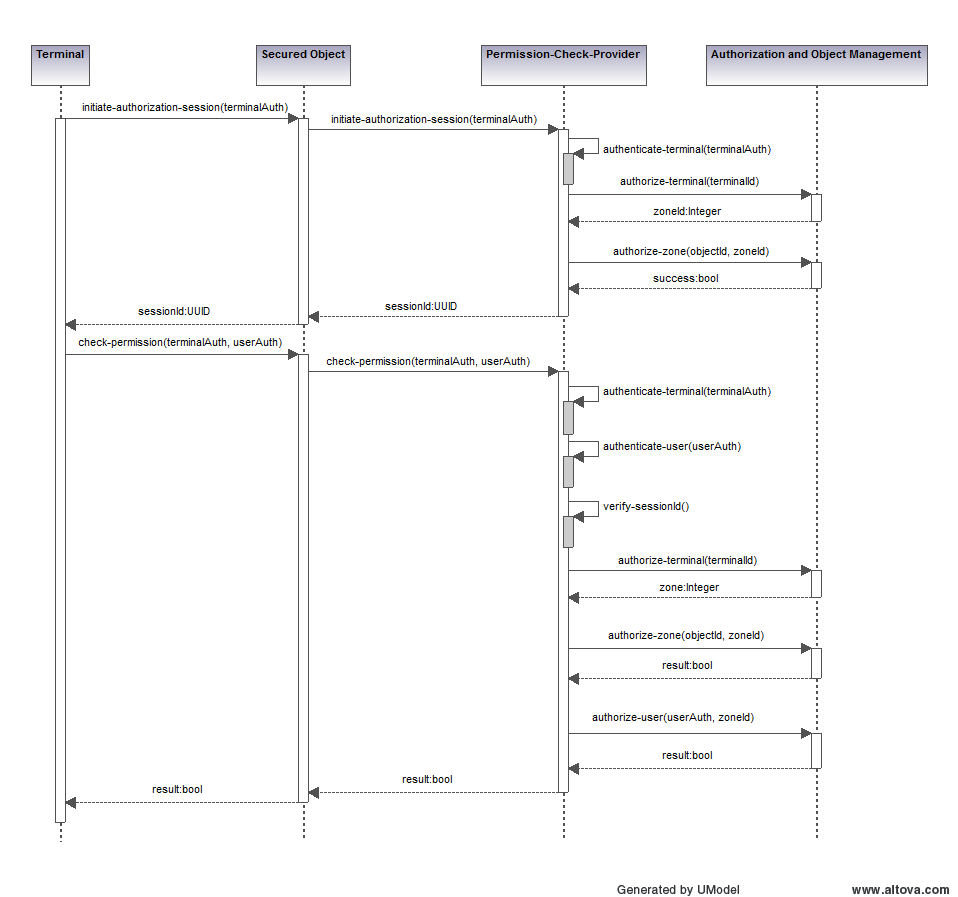
\includegraphics[width=16cm]{./imgs/sequence1.png}}
\end{figure}

The design basically consist of two phases - first a new session is initiated which results in a session ID returned to the terminal. In this step the \emph{Terminal} and the \emph{Secured Object} get authenticated and authorized by the \emph{Permission-Check-Provider}. In step two the RFID chip signs the authentication data using the stored private key and the session identifier. This information is passed on through the \emph{Secured Object} to the \emph{Permission-Check-Provider} , where a second check is performed (complete mediation). The session ID is also verified. Then the authentication data is forwarded to the \emph{Authorization and Object Management}, which decides whether to allow or deny access.

\subsubsection{initiate-authorization-session}
This method gets an \emph{InitiateSessionRequest} object passed as a parameter by the \emph{Secured Object} which contains authentication information about the source terminal. This \emph{Authentication} object keeps  the ID of the represented entity, its public certificate and some text. This information is signed using the private key. To allow a validity check the signature is stored in the object as well.

First the terminal is authenticated by checking the signature. Then the terminal and the corresponding zone get authorized by the \emph{Authorization and Object Management}. The method returns a random and system-wide unique session identifier which is used by the \emph{Permission-Check-Provider} to verify the session .

\begin{table}[h]
    \centering
    \begin{tabular}{|l|p{12cm}|} \hline
    \textbf{Source}&Secured Object\\ \hline
    \textbf{Target}&Permission-Check-Provider\\ \hline
    \textbf{Parameters}&InitiateSessionRequest (terminal:Authentication)\\ \hline
    \textbf{Authentication-Object}&id:Integer, certificate:X509Certificate, text:String, uuid: UUID (optional), signature:byte[], irisData:byte[] (optional)\\ \hline
    \textbf{Reply}&Session ID as UUID\\ \hline
    \end{tabular}
\end{table}

\subsubsection{check-permission}
Six authenticity- and authority-checks are performed in this method. The steps of \emph{initiate-authorization-session} are repeated, with the difference that a user's authentication data, attached as an \emph{Authentication} object, is also verified. Another difference is that this object also contains the  generated unique session ID and the optional iris data.

After checking the congruence of the session IDs (comparing the one signed by the user and the one previously generated) the terminal and zones are authorized by the \emph{Authorization and Object Management} again. Eventually, the authorization of the user is performed by passing on all user related information to the \emph{Authorization and Object Management}.

\begin{table}[h]
    \centering
    \begin{tabular}{|l|p{12cm}|} \hline
    \textbf{Source}&Secured Object\\ \hline
    \textbf{Target}&Permission-Check-Provider\\ \hline
    \textbf{Parameters}&PersmissionCheckRequest (terminal:Authentication, user:Authentication)\\ \hline
    \textbf{Authentication-Object}&id:Integer, certificate:X509Certificate, text:String, uuid: UUID (optional), signature:byte[], irisData:byte[] (optional)\\ \hline
    \textbf{Reply}&Boolean result\\ \hline
    \end{tabular}
\end{table}

\subsection{Secured Object}
The main purpose of the Secured Object is to forward the requests of its terminals to the \emph{Permission-Check-Provider}. Communication with the \emph{Permission-Check-Provider} and the respective terminals is secured with a certificate based SSL-encryption. Additionally we advise all external operators of these components to apply additional network based security mechanisms such as using DMZ, firewalls, VPNs or complete physical separation of the company network and the terminal-secured object network which helps to keep the target smaller.

\subsubsection{initiate-authorization-session}
Even though the secured object mainly forwards the requests to the \emph{Permission-Check-Provider}, the authenticity of the \emph{Terminal} will be checked using the signed content of the \emph{terminal} parameter. This check will be done again by the \emph{Permission-Check-Provider} (so that the terminal check cannot be bypassed by faking \emph{Secured Object}-messages) but it helps to identify problems with possibly faulty terminals earlier. If the check fails, the request is not forwarded to the \emph{Permission-Check-Provider} and after several failed authenticity checks from the same terminal, a local security officer will be informed.

\begin{table}[h]
    \centering
    \begin{tabular}{|l|p{12cm}|} \hline
    \textbf{Source}&Terminal\\ \hline
    \textbf{Target}&Secured Object\\ \hline
    \textbf{Parameters}&InitiateSessionRequest (terminal:Authentication)\\ \hline
    \textbf{Authentication-Object}&id:Integer, certificate:X509Certificate, text:String, uuid: UUID (optional), signature:byte[], irisData:byte[] (optional)\\ \hline
    \textbf{Reply}&Session ID as UUID\\ \hline
    \end{tabular}
\end{table}

\subsubsection{check-permission}
Again the content of the message is checked as far as possible before it is passed on to the \emph{Permission-Check-Provider}.

\begin{table}[h]
    \centering
    \begin{tabular}{|l|p{12cm}|} \hline
    \textbf{Source}&Terminal\\ \hline
    \textbf{Target}&Secured Object\\ \hline
    \textbf{Parameters}&PersmissionCheckRequest (terminal:Authentication, user:Authentication)\\ \hline
    \textbf{Authentication-Object}&id:Integer, certificate:X509Certificate, text:String, uuid: UUID (optional), signature:byte[], irisData:byte[] (optional)\\ \hline
    \textbf{Reply}&Boolean result\\ \hline
    \end{tabular}
\end{table}

\subsection{Terminal}
The terminals represent the only interaction point with an end user (who wants to enter a certain zone through a security door). The terminals can have different forms (e.g. passwort, iris scan ..) and can be combined with different door systems and alarm systems depending on the security.

To keep the user interaction as simple as possible, as soon as an RFID-chip is detected, the terminal will prompt for the password which is provided to the chip. The chip itself will then sign a text with its internal private key and pass that information to the terminal. This of course happens only after a successful authentication of the terminal for the chip (similar as a electronic passport does before providing any information).

If needed, the iris data is recorded at the terminal and all information including a signed text, identifying the terminal, is forwarded to the \emph{Secured Object}. While a request is pending, no additional requests can be started (other users putting an RFID-chip on the reader will be ignored). If the result is positive the door will open, if it is negative the user will be informed with a short message and the terminal will be responding to new requests again. If there is no response after a certain timeout period the request is discarded and the user has to try again.

Anticollision will be used to ensure only one RFID-chip at a time can start a request, as this will lead to problems with authentication otherwise.

\subsection{Auditing}
As the permission, object and person data is stored within separate databases, where the most important information is held historized (f.e. which persons had access to which zones and when did they have that permission). The auditing system is responsible for logging user interactions with the system. Therefore the system will log each attempt of a user trying to get access to a specific zone through a terminal, its determined outcome and the time of the event. The auditing system will not only store positive events (access granted) but also all negative outcomes and error cases (insufficient permissions, wrong pin).

The auditing data itself will also be stored in a database which makes it possible to easily access the needed data and generate reports for a manual auditing process. Of course the data is not freely accessible and every access is logged.

In addition to the log entries in the database, a second form of logging data is sent to the auditing system. This data mainly contains security related issues such as authentication failures or tarpit activations and can be used exclusively by us to perform audits about the security of our access system.

The auditing data is stored for at least three years which should be sufficient to perform security audits. As some of the objects may have additional requirements imposed by law, the access data is stored in a way that allows different storage durations for different objects.

\subsubsection{add-log-entry}
For the physical access events.

\begin{table}[h]
    \centering
    \begin{tabular}{|l|p{12cm}|} \hline
    \textbf{Source}&Permission Check Provider\\ \hline
    \textbf{Target}&Auditing\\ \hline
    \textbf{Parameters}&person:Id, terminal:Id, zone:Id, authMedia:Id, outcome:String\\ \hline
    \textbf{Reply}&none\\ \hline
    \end{tabular}
\end{table}

\subsubsection{add-log-entry}
This method is used for the logging of security related issues.

\begin{table}[h]
    \centering
    \begin{tabular}{|l|p{12cm}|} \hline
    \textbf{Source}&Permission Check Provider\\ \hline
    \textbf{Target}&Auditing\\ \hline
    \textbf{Parameters}&level:Enum, text:String\\ \hline
    \textbf{Reply}&none\\ \hline
    \end{tabular}
\end{table}

\subsection{Notification-System}
The notification system can be used to inform security personnel in cases of very specific errors (f.e. too many requests sent by a specific terminal, invalid terminals sending requests). Depending on the severity of the error, different communication channels will be used. The permission service provider will choose the appropriate communication channel to which the notification system forwards the message.

If the chosen communication channel is not available, the recipient data is not correct or the message is undeliverable an appropriate error message is returned.

\subsubsection{send-notification}
\begin{table}[h]
    \centering
    \begin{tabular}{|l|p{12cm}|} \hline
    \textbf{Source}&Permission Check Provider\\ \hline
    \textbf{Target}&Notification-System\\ \hline
    \textbf{Parameters}&channel:String, recipientIdentifier:String, serviceProvider:String, content:String\\ \hline
    \textbf{Reply}&Outcome of the operation (success/error) as String\\ \hline
    \end{tabular}
\end{table}

\section{Selected Attack Scenarios}
\subsection{Brute-Force}
One of the most common attacks against password protected systems is the brute-force or exhaustive key-search attack. This attack is a cryptanalytic attack that can (in theory) be used to break any encryption. It consists of systematically trying all possible keys until the correct key is found.

In the case an RFID-chip gets stolen or is found by an attacker, he could then start such a brute-force attack against an accounts password. One way to conduct this attack in less secure zones, where no iris scan is needed is to walk up at a terminal and iteratively try different passwords.

Our imposed system prohibits such an attack in following ways:
\begin{itemize}
   \item Once the rightful owner of a chip notices the chip missing he has the possibility to cancel the chip at the system. From this point on further login attempts with it will be denied with that device and a brute force attack will be rendered impossible.
   \item Another security feature in our system to prohibit such an attack is the implementation of the tarpit on the chip and for the \emph{Authorization and Object Management}. Once the system or the chip recognizes too many unsuccessful login attempts from the terminal, the terminal and/or the user/chip can be locked and blocked.
   \item Furthermore, the possible key range will be widened by using a strict password policy for RFID- passwords, which a user has to consider when creating or changing it.
   \item As stated, higher leveled security zones require an additional iris scan when logging in defending against brute-force (access to the eye would be necessary). 
\end{itemize}

\subsection{Shoulder-Surfing}
Another common method to obtain unknown passwords is the shoulder-surfing attack. A user standing in line at a terminal can simply watch or film another user typing a password. To prevent this, terminals will have visual covers around pin  and password pads. Furthermore no terminals will be installed closely to windows.

\subsection{Man in the Middle}
Next to brute-force attacks, Man-in-the-middle attacks (MITM) impose a serious threat to LAN and network-based systems. In computer security it is a form of active eavesdropping in which the attacker makes independent connections with the victims and relays messages between them making them believe they are talking directly to one another.

In LAN environments ARP-spoofing is a commonly used technique to achieve this. In the proposed architecture of the system, ARP-spoofing and relaying messages will be possible if a connection to the network can somehow be established. However, attackers will not have access to the content in the messages, which is ensured by the system wide SSL encryption on all communication paths.

SSL has recently been subject to attacks, which renders the protocol not 100 \% secure. For example, if an attacker has the means to obtain the root certificate from the database of a trusted certification provider, he can present this certificate to the clients during a MITM attack. Therefore clients are led to believe that the used certificate is valid and will not question its authenticity. If this is the case the attacker can decrypt the encrypted messages and gain access to their content. To decrease chances of such a successful attempt the trusted certification provider has to be chosen with care.

Another example would be stripping away the https headers from the message during a MITM attack. An attacker can simply receive encrypted content and forward it to the target as decrypted messages. Clients can notice such malicious messages, as their connection is not a https, but a http connection.When implementing SSL, users of such systems have to be made aware of these risks by some form of training. Users should additionally always check if a valid certificate is provided.

\subsection{Relay Attacks}
Relay attacks on RFID based systems oppose a serious threat because no real defense against them has been found so far. A chip of a user can be read on the fly by a close attacker. Through induction the chip in the pocket of the target can be activated and its transmitted signals can be relayed via a fast network connection to some third party trying to authorize at a terminal. The relayed signals are then used to login at the terminal. For this attack to be successfully mounted against our system an attacker has to obtain the password beforehand (through shoulder surfing or similar techniques).

\subsection{Replay Attacks}
Through a MITM attack, an attacker could record a transmitted authentication package and inject the package back into the system. Our system prevents this attack, using SSL connections creating a new session for every connection, making the packages look different for every request.

To counter a capture of a \emph{Secured Object} a new session ID is requested by the terminal at each permission request. This ID is then included in the signature created by the RFID-chip and replayed data can therefore be detected by the \emph{Permission-Check-Provider}.

\subsection{Denial of Service (DOS)}
If an RFID tag gets stolen a denial of service attack against the chip can be started. The chip can either be destroyed (using a hammer, acid or other means) or communication can be blocked by insulating the chip (through foil or other material). If the chip is then returned to the owner and manipulation is not recognized, the owner will find himself in front of terminal not getting access to the requested zone.

Because of the implementation of tar pits, proposed systems can be rendered inaccessible by simply attempting to authenticate at the system too many times with one chip. After several unsuccessful logins a user or a chip will get blocked/locked and therefore authentication is not possible until an administrator unlocks the user or the chip.

Providing possibilities to cancel a chip opposes an additional threat concerning DOS attacks. If cancellation is done via a call or an email-message an impostor could simply act like the owner of the chip, request cancellation and therefore deny the real owner access to requested zones. To prevent this, cancellation could be done requiring personal authentication and possibly providing legal documents to some administrative party.

Another possibility is to mount a blocker tag attack on an RFID reader station. For this attack an attacker places a special “blocker tag” onto the RFID reader. This tag simulates different chip Ids locking the reader through anticollision.

\subsection{Cloning a Chip}
By cloning a chip an attacker can impose as the real owner of the chip. Using RFID chips as simple hash tags this attack can easily be mounted. The systems implements a two-protocol-approach, where an additional password has to be provided with the chip during login.

\subsection{Binary Attacks}
The implementation is done using the Java Programming language. Weaknesses in current versions of the Java runtime environment have recently been exposed and successfully exploited. To minimize risks of an attacker exploiting such weaknesses only current Java versions should be used and updated in regular intervals.

Furthermore all user input and input parameters are checked before submission.


%%%%%%%%%%%%%%%%%%%%%%%%%%%%%%%%%%%%%%%%%%%%%%%%%%%%%%%%%%%%%%%%%%%%%%
%
% DO NOT CHANGE THE FOLLOWING PART
%
%%%%%%%%%%%%%%%%%%%%%%%%%%%%%%%%%%%%%%%%%%%%%%%%%%%%%%%%%%%%%%%%%%%%%%

\end{document}


